\begin{center}
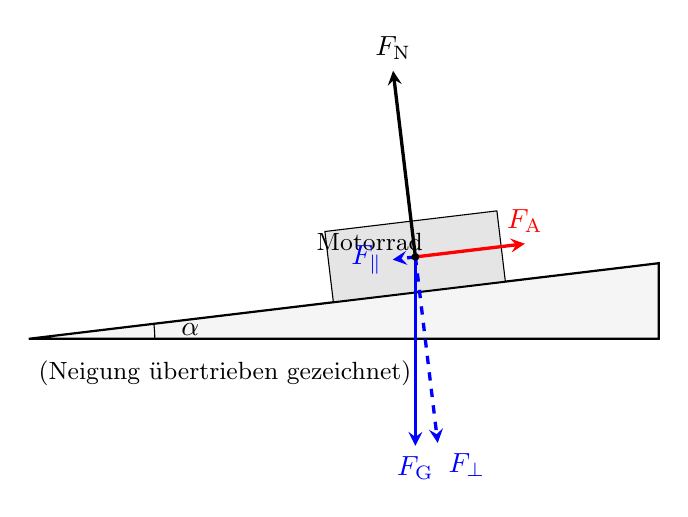
\begin{tikzpicture}[>=stealth]
 \draw[thick, fill=gray!8] (0,0) -- (8.00,0) -- (8.00,0.96) -- cycle;
 \draw (1.6,0) arc (0:6.84:1.6);
 \node at (2.05,0.12) {$\alpha$};
 \begin{scope}[shift={(4.96,0.60)}, rotate=6.84]
  \draw[fill=gray!20] (-1.1,0) rectangle (1.1,0.9);
  \node[font=\small] at (-0.55,0.70) {Motorrad};
 \end{scope}
 \draw[->, very thick, blue] (4.91,1.04) -- ++(-90.00:2.40) node[anchor=north] {$F_\mathrm{G}$};
 \draw[->, very thick, blue, dashed] (4.91,1.04) -- ++(-83.16:2.38) node[anchor=north west] {$F_\perp$};
 \draw[->, very thick, blue, dashed] (4.91,1.04) -- ++(186.84:0.29) node[anchor=east] {$F_\parallel$};
 \draw[->, very thick, black] (4.91,1.04) -- ++(96.84:2.38) node[anchor=south] {$F_\mathrm{N}$};
 \draw[->, very thick, red] (4.91,1.04) -- ++(6.84:1.40) node[anchor=south] {$F_\mathrm{A}$};
 \fill (4.91,1.04) circle (0.05);
 \node[anchor=north west, font=\small] at (0,-0.15) {(Neigung übertrieben gezeichnet)};
\end{tikzpicture}
\end{center}

Die Steigung $p = \stgO$ ist das Verhältnis von Höhe zu horizontaler Strecke, also $\tan\alpha = p$ und
\begin{align}
 \alpha &= \wiF = \wi
\end{align}
Die Beschleunigung in der Zeit $t = \tMoO$ ist
\begin{align}
 a &= \aMoF = \frac{\vEn-\vAn}{\tMo} = \aMo
\end{align}
Reibung und Luftwiderstand werden vernachlässigt. Entlang des Hangs wirken die Antriebskraft $F_\mathrm{A}$ hangaufwärts und die Hangabtriebskraft $F_\parallel = m\,g\sin\alpha$ hangabwärts. Nach dem Aktionsprinzip gilt
\begin{align}
 F_\mathrm{A} - m\,g\sin\alpha &= m\,a
\end{align}
und damit
\begin{align}
 F_\mathrm{A} &= \FAnF \\
   &= \mMo\cdot\left(\aMo+\gE\cdot\sin\left(\wi\right)\right) \\
   &= \FAn \approx \result{\FAnP{0}{2}}
\end{align}
